\section{Data and experiments}
\label{sec:experiments}
%
\subsection{Shape prior}
%
As described in \autoref{sec:introduction}, the general situation in
the connectivity pipelines consists of having 
a reliable segmentation obtained from the high resolution \ac{t1} 
reference image. Therefore, a precise location of the tissue interfaces
of interest is available in a reference space. Given that the anatomical 
reference segmentation is beyond the scope of this manuscript, we simply 
rely on the shape priors obtained from the models.
%
\subsection{Synthetic gray-scale data}
%
The first, toy example is inspired by a problem shown for coupled CSF/GM and GM/WM segmentation in \citep{macdonald_automated_2000}. These authors note that ``partial volume effects blur the distinction between closely adjacent surfaces in deep sulci, leading to a well-known segmentation error in which the deeper reaches of sulci are not penetrated by the putative surface model.'' This problem is aggravated in DWI, since the resolution tends to be worse compared to the anatomical images considered in \citep{macdonald_automated_2000}. They test their coupled segmentation algorithm on an image, ``representing a sulcus in which the distinction between opposing banks of the sulcus has been obscured by partial volume.''  Here, we have reproduced a very similar model. As illustrated in \autoref{fig:sulcusmodel}, conventional single surface segmentation of the CSF/GM boundary misses to capture the sulcus in its full depth. With our proposed model, we expect the joint segmentation-registration to be driven largely by the inner, GM/WM contour that exhibits sufficient contrast and lesser partial volume effects. The shape prior of the outer, difficult contour will then be co-aligned through the regularity of the estimated deformation field.

\begin{figure}
\begin{tabular}{ccccc}
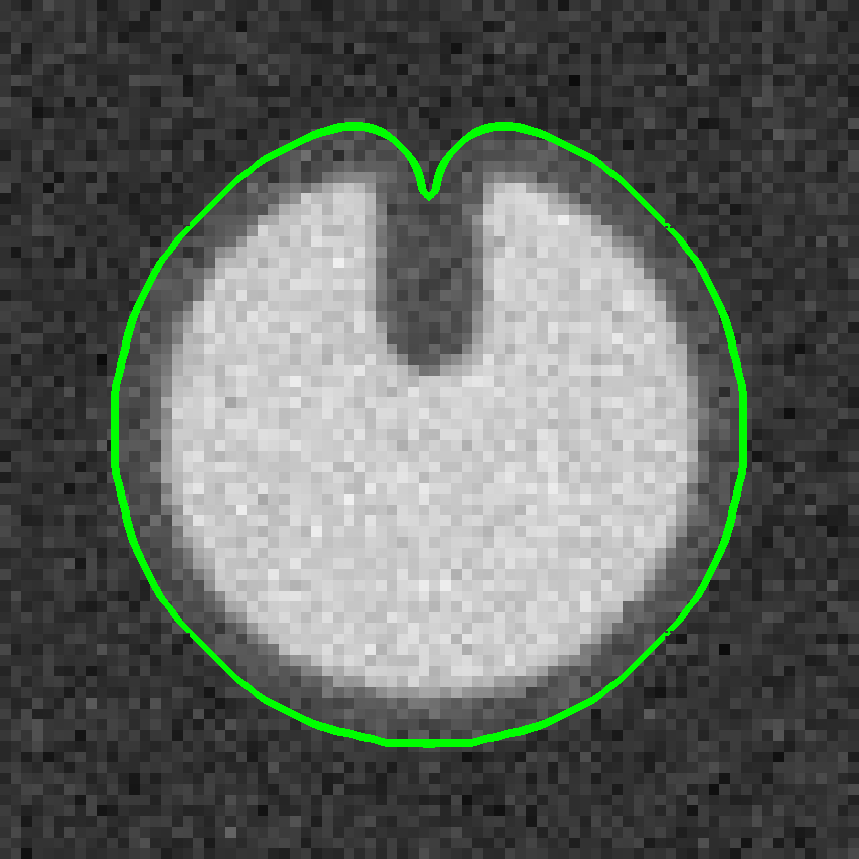
\includegraphics[width=0.19\textwidth]{contours_wrong} & 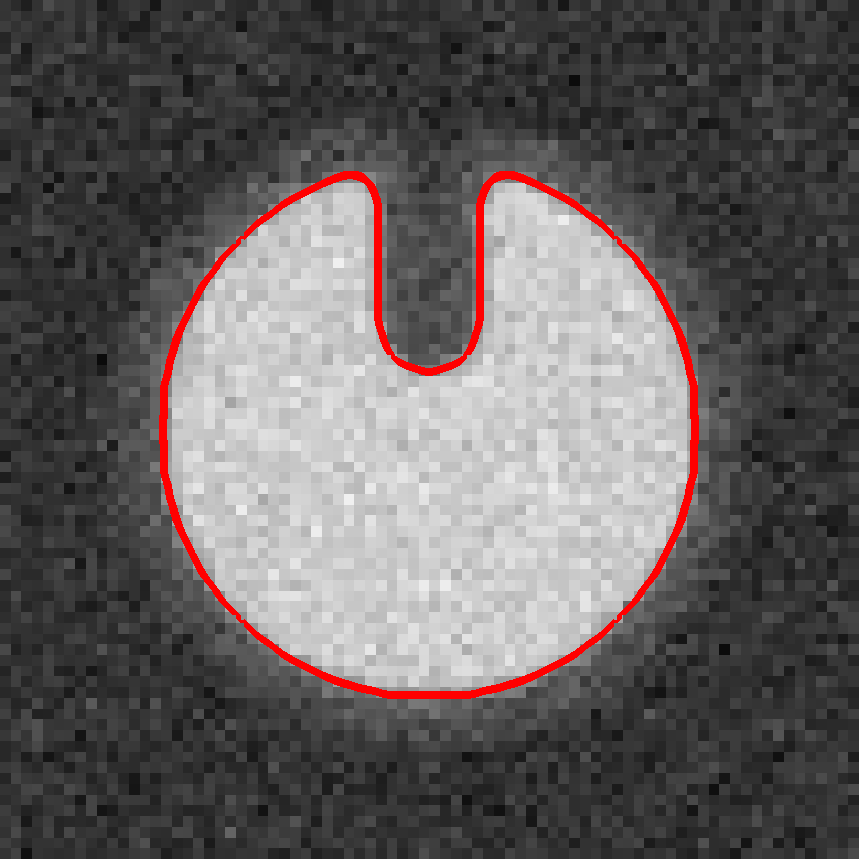
\includegraphics[width=0.19\textwidth]{contours_inner} &
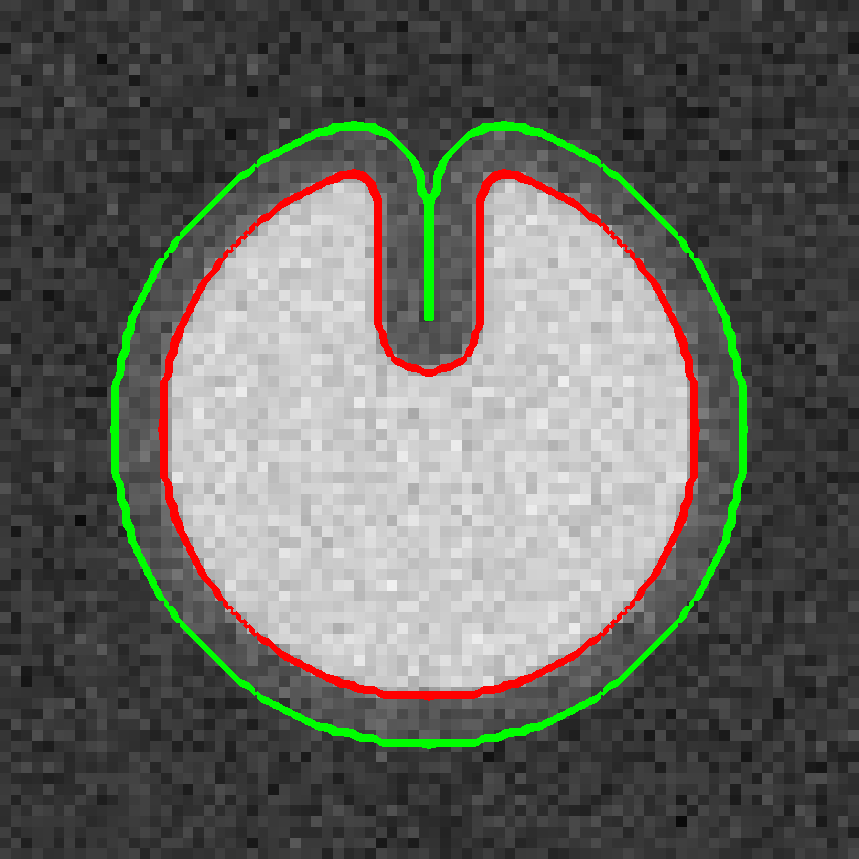
\includegraphics[width=0.19\textwidth]{contours_both} &
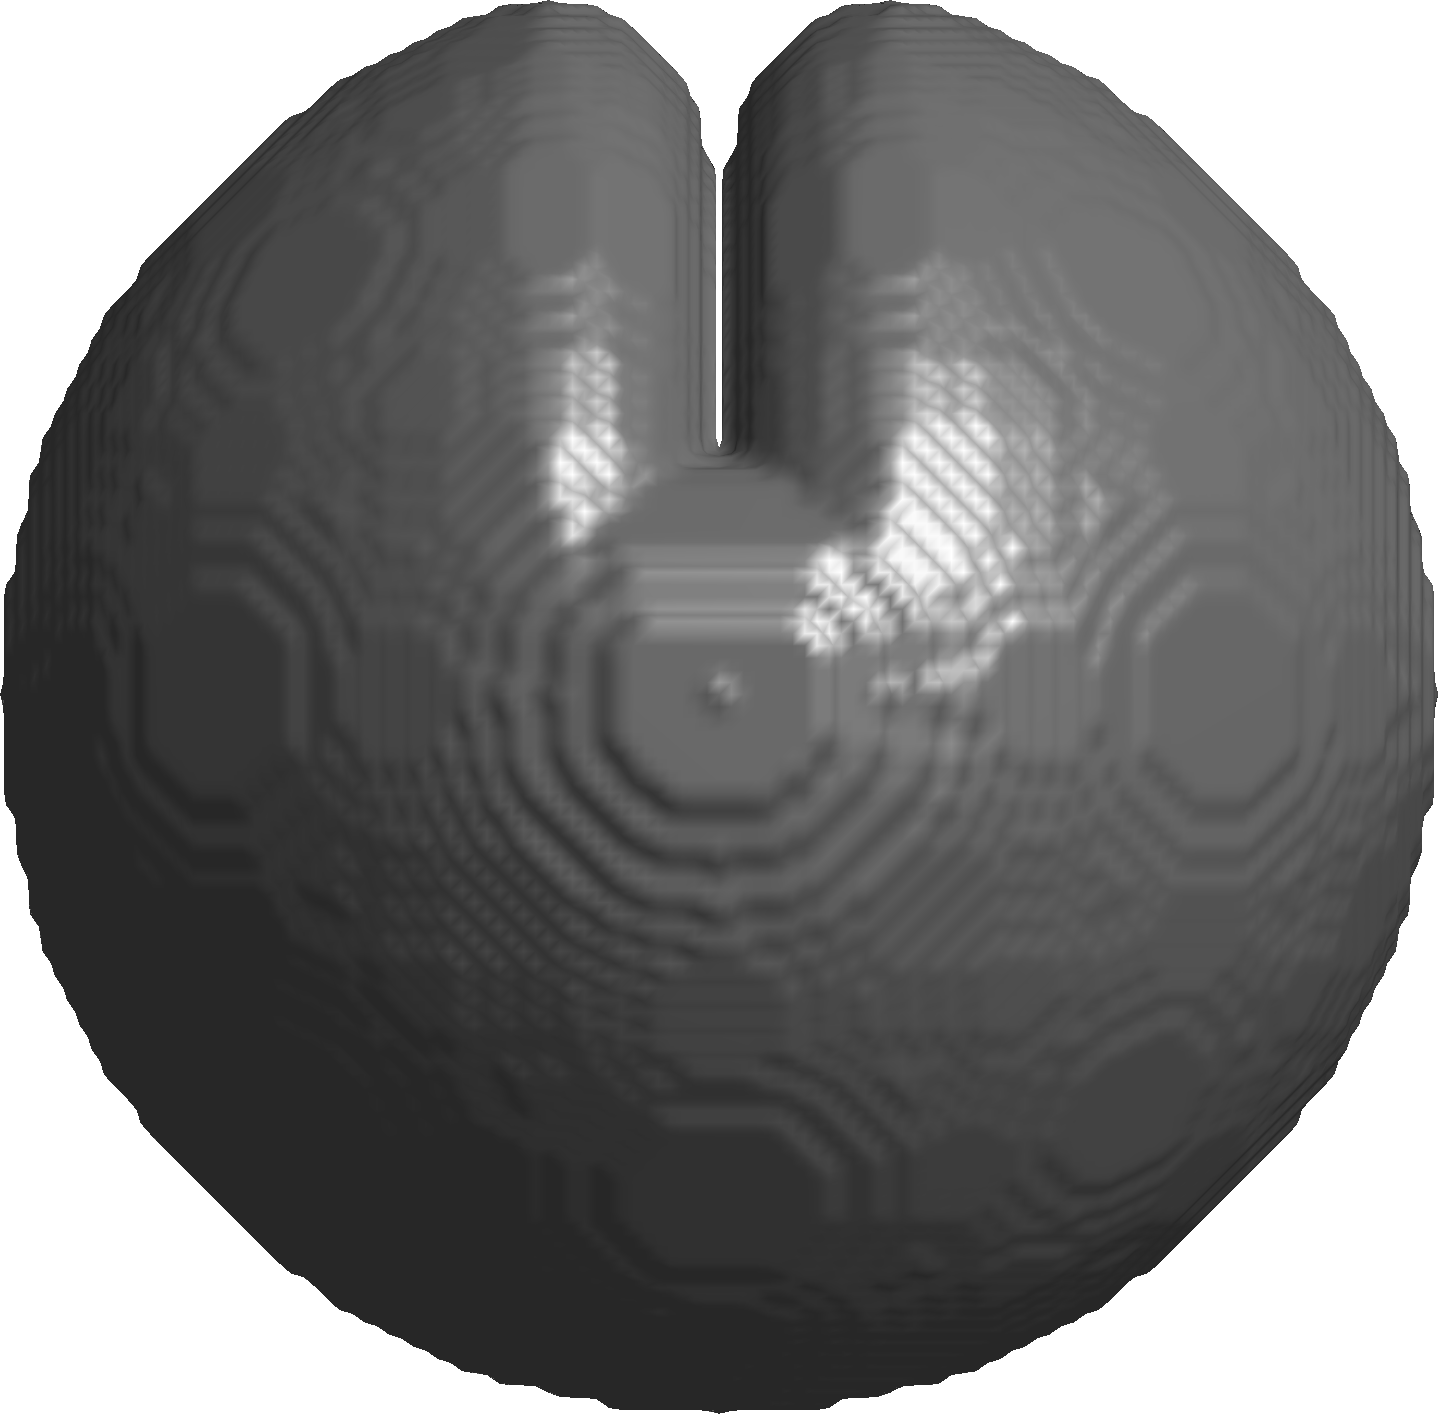
\includegraphics[width=0.19\textwidth]{pialsurf} &
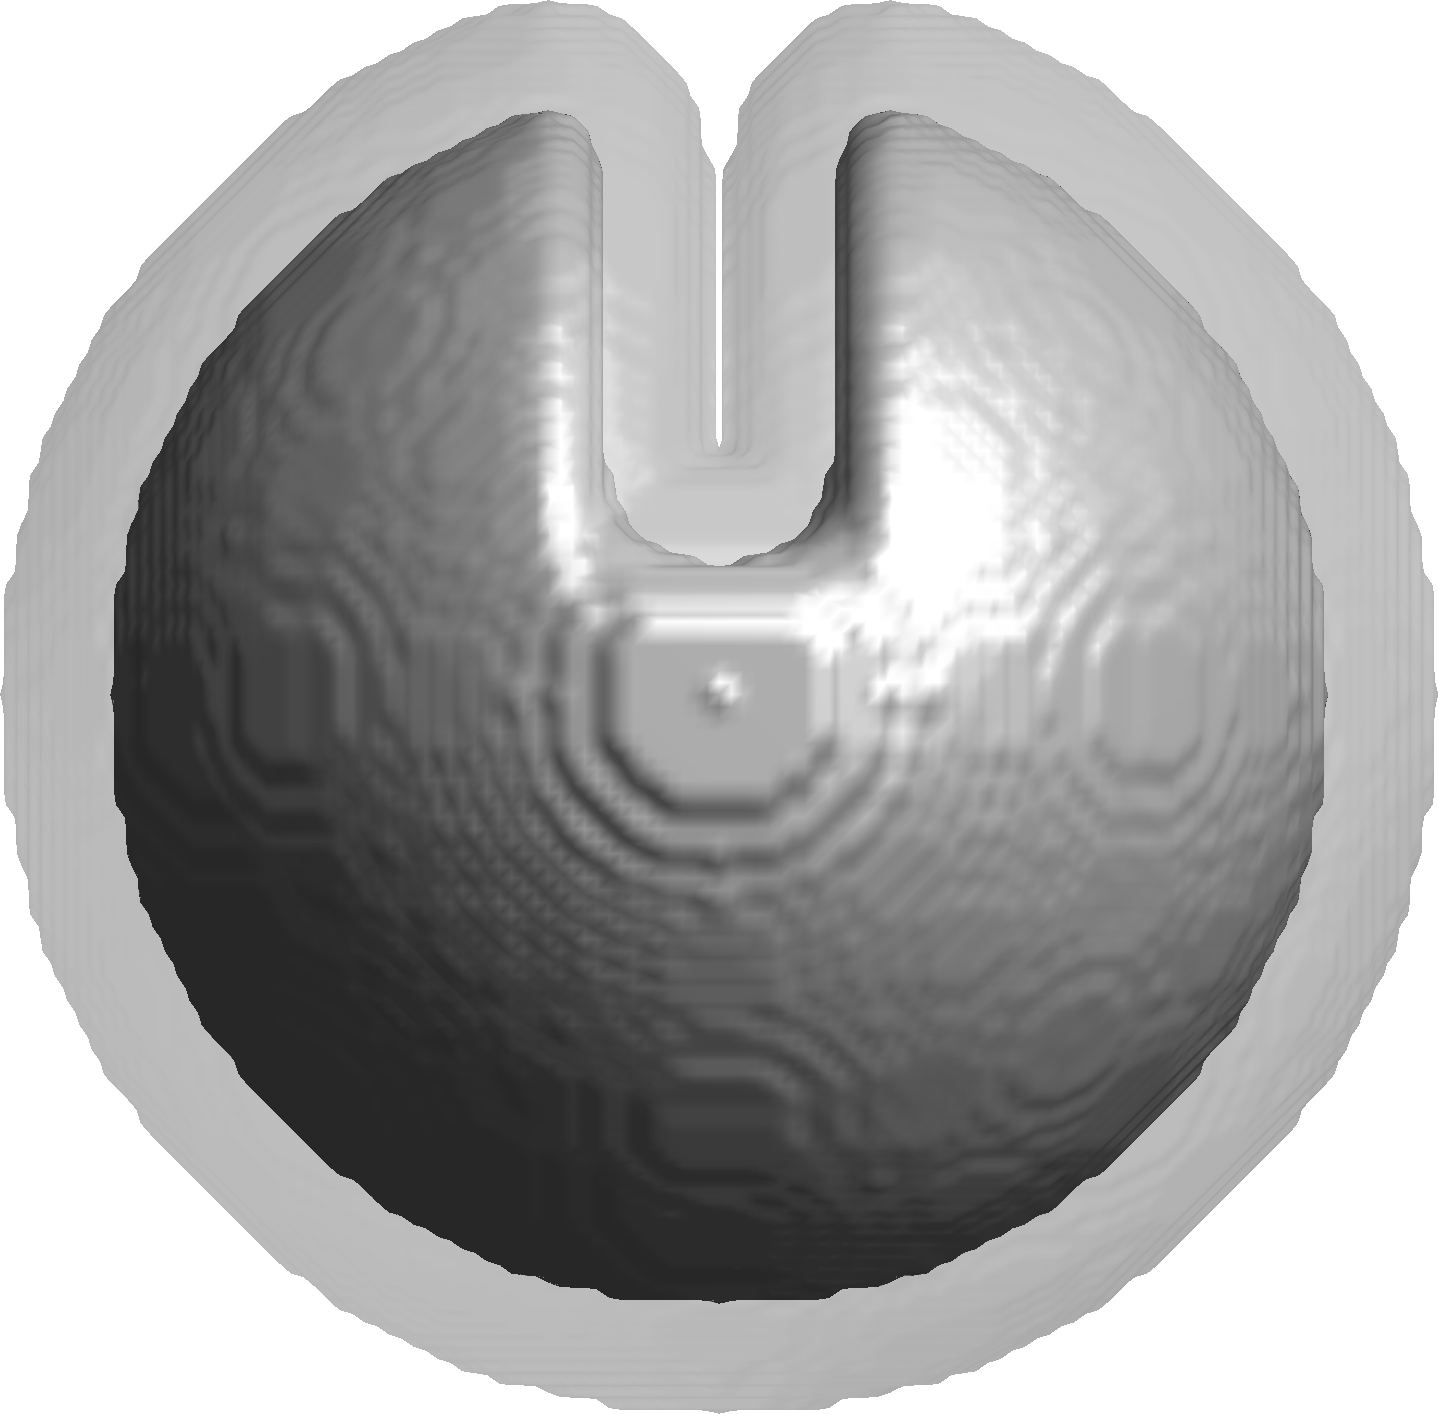
\includegraphics[width=0.19\textwidth]{gmwmsurf}\\
a)&b)&c)&d)&e)
\end{tabular}
\caption{The gray-scale sulcus model. a) The apparent CSF/GM boundary is affected by partial volume in the sulcal cavity, and conventional segmentation is likely to miss it. b) The GM/WM interface here has consistently good contrast. c) Registering the two shape priors coupled through deformation field regularity is expected to guide the CSF/GM contour. d\&e) 3D view of the two shape priors.}
\label{fig:sulcusmodel}
\end{figure}

%
\subsection{Simulated diffusion data}
%
In order to demonstrate the functionality of the methodology, 
and characterize its possibilities with diffusion data,
we simulated the \acs{dw} signal of a synthetic phantom from a model
consisting of several spherical shapes emulating
the different brain tissues (see \autoref{fig:fa}, first row). 
We reconstructed the signal with standard procedures to 
approximate the environment to the real one at maximum. \\

\paragraph{Signal simulation}
To numerically simulate the MRI signal attenuation when applying a diffusion 
gradient in a voxel with $N$ fiber populations we made use of the standard 
\emph{Multi-Tensor Model}~\cite{Tuch:2002aa}:
%
\begin{equation} 
\label{eqn:MultiTensor}
S(\vec{q}) / S_{0} = \sum_{i=1}^{N} f_{i} \, \exp{ \left( -b \, \vec{q}^{T} \, \mathbf{D}_i \, \vec{q}\right) } + f_{iso} \, \exp{ \left( -b \, \mathbf{D}_{iso} \right) } ,
\end{equation}
%
where $\vec{q} \in \mathbb{S}^2$ is the direction of the diffusion gradient 
applied, $b$ is the b-value accounting for its strength, $S_0 \equiv S(\vec{0})$ 
is the signal with no diffusion weighting, $f_i$ and $\mathbf{D}_i$ are 
respectively the volume fraction and the diffusion tensor characterizing the 
$i$-th fiber population.

The diffusion tensors $\mathbf{D}_i$ and $\mathbf{D}_{iso}$ describe the diffusion 
processes of each fiber compartment and of contaminations from the CSF. In this work, 
these quantities have been taken from standard ranges typically observed in the 
human brain~\cite{Canales-Rodriguez:2009aa}.

\paragraph{Noise simulation}
The diffusion MRI signal $S$ has been corrupted with 
\textit{Rician noise}~\cite{Gudbjartsson:1995aa} as follows:
%
\begin{equation}
	\tilde{S} = \sqrt{ (S + \varepsilon_1)^2 + \varepsilon_2^2 }
\end{equation}
%
where $\varepsilon_{1,2}$ are Gaussian distributed with zero mean
and standard deviation $\sigma = S_0 / \mathit{SNR}$ and \acs{snr}
is the \ac{snr} on the $S_0$ image.

\paragraph{Derived scalar features}
The target \ac{dwi} data is characterized by its distortions and its
low resolution (typically around $2.2x2.2x3mm^3$). Depending on the
posterior reconstruction methodology and the angular resolution
intended, the \ac{dwi} raw data has to be processed in order to
extract the information in a manageable manner. The properties of
the reconstructed tensors and derived scalar maps have been
studied by \cite{ennis_orthogonal_2006}. Based on their
findings, the proposed energy model adapts to the \ac{fa} and \ac{md}
for their properties. Whereas \ac{fa} describes the \emph{shape} of diffusion, 
the \ac{md} depicts the \emph{magnitude} of the process. 

\textbf{FIXME: can you give the respective formula, how you get from the above signal to FA/MD?}
\begin{equation}
FA = \sqrt{ \frac{3}{2}},\frac{\sqrt{ (\lambda_1 - \hat{\lamda})^2 + (\lambda_2 - \hat{\lamda})^2 + (\lambda_3 - \hat{\lamda})^2}}{\sqrt{ {\lambda_1}^2 + {\lambda_2}^2 + {\lambda_3}^2}}
\end{equation}

There exist two main reasons to justify their choice. 
First, they are well-understood and standardized in clinical routine.
Second, together they contain most of the information that is
usually extracted from the \ac{dwi}-derived scalar maps. \\

\subsubsection{Simulated distortions}

For this model, we created manually a sound distortion visually similar
to real \ac{epi} distortions. We interpolated the distortion to a 
dense deformation field, necessary for warping the raw \ac{dwi} simulated
data. Once the signal was deformed, we proceeded to reconstruct the
\ac{dti} and subsequently obtained the scalars of interest (\ac{fa}, \ac{md}).
Finally, we estimated their parameters using the tissue probability
distribution maps from the original model (\autoref{table:parameters}).

\begin{table}
\begin{tabularx}{1.0\textwidth}{c|XXX}
\hline
         & $\mathbf{\mu}_{FA}$ & $\mathbf{\mu}_{MD}$ & $\Sigma$ \\
\hline
\ac{wm}  & 0.778 & 6.94\e{-4} & 
   $\begin{pmatrix}
   	4.85\e{-3} & -6.90\e{-6} \\ -6.90\e{-6} & 1.03\e{-8}
   \end{pmatrix}$
\\
\hline
\ac{gm}  & 0.119 & 8.95\e{-4} &
   $\begin{pmatrix}
   	5.90\e{-4} & -1.43\e{-6} \\ -1.43\e{-6} & 1.04\e{-8}
   \end{pmatrix}$
\\
\hline
\ac{csf} & 0.103 & 2.99\e{-3} &
   $\begin{pmatrix}
   	1.19\e{-3} & 2.22\e{-7} \\ 2.22\e{-7} & 1.56\e{-8}
   \end{pmatrix}$
\\
\hline
\end{tabularx}
\caption{Model parameters}
\label{table:parameters}
\end{table}
